Also wird hier ausgetestet was passiert, wenn nicht kaskadiert wird. Da dies nur dann gut geht, wenn TF nicht verwendet wird, wird alles direkt 
auf dem Targetdatensatz gelernt. Die Netze werden so verändert, dass sie insgesamt gleich viele Hiddenlayer wie alle kleinen Netze, die im 
Direct Cascade Verfahren vorkommen, zusammen haben. Es werden dabei auch gleich viele Epochen insgesamt benutzt wie eben gerade. 

\begin{figure}[htpb]
    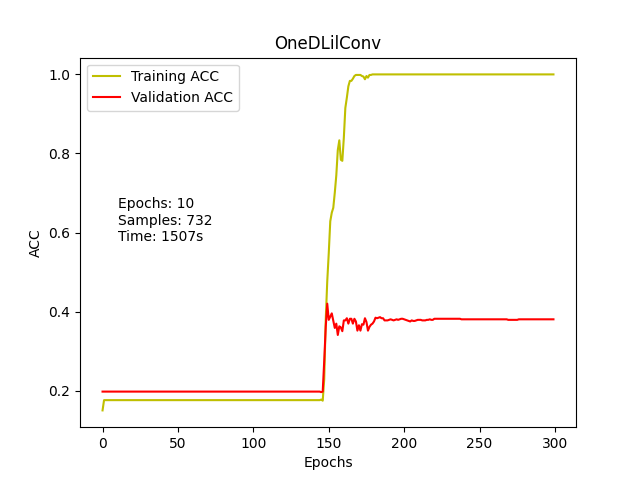
\includegraphics[height=5cm]{../../Plots/ba_plots/classnocascade/1dc.png}
    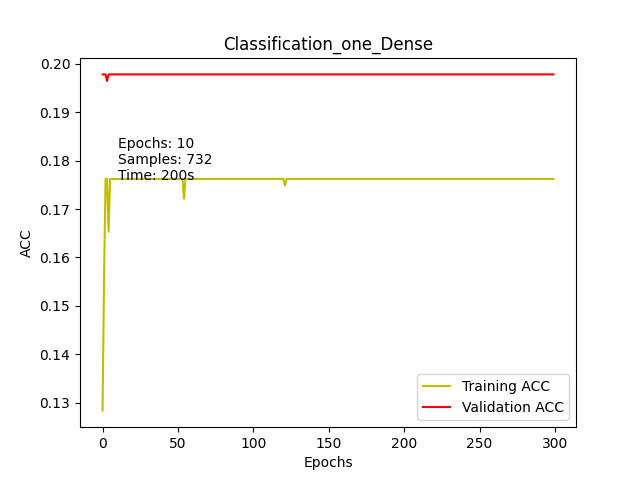
\includegraphics[height=5cm]{../../Plots/ba_plots/classnocascade/cod.png}
    \caption{\label{fig:nocascade} Netze ohne Kaskadierung}
\end{figure}

% Das dürfte daran liegen, dass zu diesem Zeitpunkt die Gewichte des Netzwerkes ausreichend aktualisiert worden sind, dass die Vordersten ebenfalls 
% in die richtige Richtung verändert werden. 

Was in der Figure 4.6 auffällt ist, dass es bei den meisten Epochen zu keinem Lerneffekt kommt. Ebenso kommt Overfitting vor, was bei so wenigen 
Daten zu erwarten ist. Obwohl es hier nicht TF angewendet wird, gibt es in der Mitte des einen Plot einen plötzlichen Anstieg der Accuracy. 
Der Start dieser Verbesserung kam davon, dass der Validationwert minimal schlechter wurde. Des Wegen 
scheint es zudem so, dass es zu einem lokalen Minimum während des Trainings gekommen ist. Bei dem anderen Netz blieb der Wert auf dem des 
lokalen Minimums stehen, denn es sind die exakt gleichen Werte. Trotzdem wird durch Figure 4.6 klar, dass es bei so wenigen Daten eine maximale 
Accuracy von 40\% zu erwarten ist. An diese kommt weder die Version des nur Kaskadierens noch die des Kaskadierens mit TF auch nur 
ansatzweise heran. Diese haben einen maximalen Wert von 20\% und sind somit nur halb so gut. 

Daraus folgt, dass es bereits an der Kaskadierung liegt, dass Klassifikation sinnlos mit TF in dem Direct Cascade Verfahren ist. 
